\chapter{A unifying logic for the Semantic Web}
\section{The vision of the Semantic Web}
My idea for this chapter is to explain a little bit more about the semantic web in general and its architecture


\section{Architecture}

Gerber \cite{Gerber} \cite{Gerber2}. Really nice: abstracts from technnologies. Bad: the word ``unifying Logic'' dissapeared.

\cite{rearch} Paper by Boley, Kifer, etc. ``realistic'' architecture, not just one technology. 

\begin{figure}[h!]
	\centering
	%\begin{adjustwidth}{-\marginnotewidth}{}%
	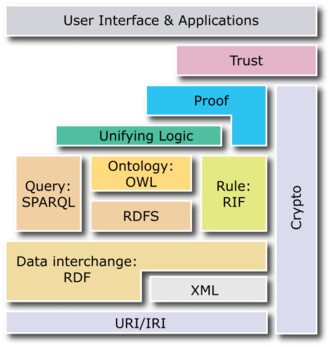
\includegraphics{Semantic_Web_Stack}
	%\end{adjustwidth}
	\caption{Semantic Web Stack. Source: \url{https://www.w3.org/2007/03/layerCake.svg}}
	\label{fig:stack}
\end{figure}
\subsection{Data Interchange}
RDF

\cite{rdf}
\subsection{Querying}
\subsection{Ontologies}
RDFS
OWL
\subsection{Rule Based Logics}
RIF

SWRL

N3

\cite{N3Logic}

\subsection{Unifying Logic}
What do we expect from the ``unifying logic''?

The vision of the Semantic Web is to enable machines to use the Web just as humans do. For that they need to be able to \emph{understand} and \emph{exchange} data through the Web. 
An unambiguous way to express knowledge is needed, a logic. 
This logic needs to be well defined to avoid misunderstandings and it needs to be agreed on this definition between all possible parties involved.


Also say why you should go for N3: unifying logic is not just a theoretical construct, it also gives practical advantages: reasoning is often faster when you use only one logic.  
It has advantages if you need 
the features of different frameworks. Of course, if you know that, eg only querying is needed you should still go for SPARQL.


% The Unifying Logic needs to be well-defined in itself, it needs to be able to ``understand'' the underlying formats, in particular to query, do DL reasoning and use rules. 
% Additionally it should provide the opportunity to connect to the proof layer.
Requirements:
\begin{description}
 \item[clear semantic definition] 
The meaning of every statement needs to be clearly defined.
 \item[compatibility with existing Web standards]  Existing standards of the Semantic Web need to be supported. 
 In particular, querying, Description Logics, and rule based reasoning need to be covered.
 \item[support of proofs] It must be possible to express, interchange and check all derivations made in the logic.
 \item[capability to handle change] It must be possible to express and reason about change.
\end{description}
\subsection{Proofs}
\section{Research questions}
Question: Is N3 a suitable candidate to become the unifying logic for the semantic web?

Sub-questions:

Can we give a clear semantic definition of Notation3 Logic?

How does Notation3 Logic interfere with other formats? Can SPARQL, OWL and RIF be expressed?

Is it possible to express proofs in N3?

Can N3 handle change?

I think I need to be more specific. To find that: what do I actually do here?

\textbf{Part 1:}
I try to find out what the semantics of N3 is. 

I find one specific problem which is not easy to solve: implicit quantification. Here I need to discuss the problem: meaning not clear.

Next: who understands it how? Different ``official'' sources, tests on reasoners.


Then: we know the differences, can we fomalize those?

To do so, we go for attribute grammars, implemet a tool, test the impact of the problem.

We argue that we are in favor of doing as EYE does, but for the rest of the thesis we assume the semantics as in the team submission. Following that, we also give a direct semantic which we want 
to use in the following chapters.

Question: should I display both, direct and elaboration Semantics? Alternative: only go for elaboration, but then the proofs in the RESTdesc part need to be adjusted.

Conclusion: N3 is, as we will see a very nice logic. To be used in the web, a better semantics is needed. 

\textbf{Part 2:}
N3 and other standards.

The idea of this chapter is to illustrade on practical cases that tasks which were already implemented by different frameworks can be taken over by N3. We have two use cases: 

Firstly, a nurse call system. Here, a solution was implemented in OWL DL using SPARQL on top of it. We show that N3 can be use to combine the parts of DL relevant for this approach SPARQL queries. 
The reasoning times of both systems are then compared. We also discuss steps to further improve performance of reasoning.  


A: owl

Show that OWL RL is quite powerful (first ORCA paper).
 - introduce use case
Show that reasoning can be optimized with precomputation.

Dhort new part that we can go beyond OWL RL, say why, but: futere work

B: querying and RIF
example constraints paper (need to think about that part).

\textbf{Part 3:}

N3 and proofs

First: it is possible to express proofs in N3: introduce the calculus.

Second: it is a very nice feature even beyond the obvious use of ``trust''. To show that, we introduce two practical applications

A: Pragmatic proof: we describe Web APIs using N3 rules. Then we can use proofs to combine these. Has been used for many applications. Problem: no way to express change
B: Sensdesc: same idea as RESTdesc but in a different setting: we cuse rules to describe possible queries to streams. Then we can use the proof to determine whether a query is relevant for a request.

Conclusion: The feature ``proof'' is very useful. For some use cases N3 has limits.

\textbf{Part 4: going beyond the limits}

introduce weighted transition logic to express change

This part is optional



Somewhere I need to talk about problems, especially decidability and for example the problems of OWL full.